\documentclass[a4paper]{article}
\usepackage{cmap}
\usepackage[utf8]{inputenc}
\usepackage[T2A]{fontenc}
\usepackage[english,russian]{babel} 
\usepackage[left=15mm, top=15mm, right=15mm, bottom=30mm, nohead, nofoot]{geometry}
\usepackage{blindtext}  % рыба-текст
\usepackage{graphicx}  % изображения
\usepackage{float} % плавающие объекты
\usepackage{wrapfig}  % изображения
\usepackage{tikz} % графика
\usepackage{mdframed} % рамки
\usepackage{xcolor} % определение цветов
\usepackage{nicefrac} % красивые дроби
\usepackage{cancel} % сокращение
\usepackage{amsmath,amsfonts,amssymb} % математический пакет
\usepackage{hyperref}  % гиперссылки
\usepackage{fancybox,fancyhdr} % хедер и футер
\usepackage{listings} % код
\usepackage[skip=2pt]{caption} % расстояние между подписью и картинкой
\pagestyle{fancy}
\fancyhf{}
\fancyhead[L]{Лабораторная работа №6}
\fancyhead[R]{\textit{Влияние нулей и полюсов передаточной функции на динамические свойства}}
\fancyfoot[C]{\thepage}
\headsep=4mm
\footskip=13mm
\setlength{\parindent}{0em}
\setlength{\parsep}{0em}
\setlength{\headheight}{12pt}
\setlength{\topmargin}{-38pt}
\setlength{\arraycolsep}{2pt}

\definecolor{urlcolor}{HTML}{3454D1}
\definecolor{linkcolor}{HTML}{3454D1}
\hypersetup{
    pdfstartview=FitH,
    linkcolor=linkcolor,
    urlcolor=urlcolor,
    colorlinks=true,
    pdftitle={Лабораторная работа №6},
    pdfauthor={Овчинников П.А.}
}

\definecolor{strings}{rgb}{0,0.6,0}
\definecolor{comments}{rgb}{0,0.3,0}
\definecolor{numbers}{rgb}{0.5,0.5,0.5}
\definecolor{keywords}{rgb}{0.09,0.61,0.95}
\definecolor{background}{rgb}{0.97,0.97,0.97}
\lstdefinestyle{codestyle}{
    backgroundcolor=\color{background},
    commentstyle=\color{comments},
    keywordstyle=\color{keywords},
    stringstyle=\color{strings},
    numberstyle=\tiny\color{numbers},
    basicstyle=\ttfamily\footnotesize,
    breakatwhitespace=false,
    breaklines=true,
    captionpos=b,
    inputencoding=utf8,
    keepspaces=true,
    numbers=left,
    numbersep=5pt,
    showspaces=false,
    showstringspaces=false,
    showtabs=false,
    tabsize=2,
    extendedchars=true,
    literate=
    {а}{{\cyra}}1
    {б}{{\cyrb}}1
    {в}{{\cyrv}}1
    {г}{{\cyrg}}1
    {д}{{\cyrd}}1
    {е}{{\cyre}}1
    {ж}{{\cyrzh}}1
    {з}{{\cyrz}}1
    {и}{{\cyri}}1
    {й}{{\cyrishrt}}1
    {к}{{\cyrk}}1
    {л}{{\cyrl}}1
    {м}{{\cyrm}}1
    {н}{{\cyrn}}1
    {о}{{\cyro}}1
    {п}{{\cyrp}}1
    {р}{{\cyrr}}1
    {с}{{\cyrs}}1
    {т}{{\cyrt}}1
    {у}{{\cyru}}1
    {ф}{{\cyrf}}1
    {х}{{\cyrh}}1
    {ц}{{\cyrc}}1
    {ч}{{\cyrch}}1
    {ш}{{\cyrsh}}1
    {щ}{{\cyrshch}}1
    {ъ}{{\cyrhrdsn}}1
    {ы}{{\cyrery}}1
    {ь}{{\cyrsftsn}}1
    {э}{{\cyrerev}}1
    {ю}{{\cyryu}}1
    {я}{{\cyrya}}1
    {А}{{\CYRA}}1
    {Б}{{\CYRB}}1
    {В}{{\CYRV}}1
    {Г}{{\CYRG}}1
    {Д}{{\CYR96}}1
    {Е}{{\CYRE}}1
    {Ж}{{\CYRZH}}1
    {З}{{\CYRZ}}1
    {И}{{\CYRI}}1
    {Й}{{\CYRISHRT}}1
    {К}{{\CYRK}}1
    {Л}{{\CYRL}}1
    {М}{{\CYRM}}1
    {Н}{{\CYRN}}1
    {О}{{\CYRO}}1
    {П}{{\CYRP}}1
    {Р}{{\CYRR}}1
    {С}{{\CYRS}}1
    {Т}{{\CYRT}}1
    {У}{{\CYRU}}1
    {Ф}{{\CYRF}}1
    {Х}{{\CYRH}}1
    {Ц}{{\CYRC}}1
    {Ч}{{\CYRCH}}1
    {Ш}{{\CYRSH}}1
    {Щ}{{\CYRSHCH}}1
    {Ъ}{{\CYRHRDSN}}1
    {Ы}{{\CYRERY}}1
    {Ь}{{\CYRSFTSN}}1
    {Э}{{\CYREREV}}1
    {Ю}{{\CYRYU}}1
    {Я}{{\CYRYA}}1
}
\lstset{style=codestyle}

\addto\captionsrussian{
  \renewcommand{\contentsname}
    {\centering Содержание}
}
\newcommand{\addsection}[1]{
    \phantomsection
    \addcontentsline{toc}{section}{#1}
    \section*{\centering #1}
}
\newcommand{\addsubsection}[1]{
    \phantomsection
    \addcontentsline{toc}{subsection}{#1}
    \subsection*{\centering #1}
}
\newcommand{\addsubsubsection}[1]{
    \phantomsection
    \addcontentsline{toc}{subsubsection}{#1}
    \subsubsection*{\centering #1}
}

\newmdenv[
    leftmargin = 0.5em,
    skipabove = 0.5em,
    skipbelow = 0.5em,
    linewidth = 1pt,
    rightline = false,
    topline = false,
    bottomline = false
]{quotebox}

\newlength{\tempheight}
\newcommand{\Let}{
\mathbin{\text{\settoheight{\tempheight}{\mathstrut}\raisebox{0.4\pgflinewidth}{
\tikz[baseline=0.5ex,line cap=round,line join=round] \draw (0,0) --++ (0.3em,0) --++ (0,2.3ex) --++ (-0.3em,0);
}}}}
\newcommand*\squared[1]{\tikz[baseline=(char.base)]{
            \node[shape=rectangle,draw,inner sep=4pt] (char) {#1};}}
\newcommand*\msquared[1]{\tikz[baseline=(char.base)]{
            \node[shape=rectangle,draw,inner sep=4pt] (char) {$\displaystyle #1$};}}
\newcommand\argmax[1]{\underset{#1}{\text{argmax}}}
\renewcommand\max[1]{\underset{#1}{\text{max}}}
\newcommand{\at}{\biggr\rvert}
\newcommand{\shiftright}[3]{\makebox[#2][r]{\makebox[#1][l]{#3}}}
\newcommand{\e}{\;\text{e}}
\let\oldint\int
\def\int{\oldint\limits}
\DeclareRobustCommand{\divby}{%
  \mathrel{\vbox{\baselineskip.65ex\lineskiplimit0pt\hbox{.}\hbox{.}\hbox{.}}}%
}

\newcommand\NB{\textbf{N\kern-0.32em\textcolor{red}{B}}}

\begin{document}
\begin{titlepage}
    \begin{center}
    \includegraphics[width=0.18\textwidth]{~/Изображения/itmo_logo.png}\\[10pt]
        Федеральное государственное автономное образовательное \\ учреждение высшего образования \\[6pt]
        САНКТ-ПЕТЕРБУРГСКИЙ НАЦИОНАЛЬНЫЙ \\ ИССЛЕДОВАТЕЛЬСКИЙ УНИВЕРСИТЕТ ИТМО \\[16pt]
        Факультет систем управления и робототехники \vfill
        {\large Лабораторная работа №6} \\[0.5em]
        {\large \textbf{\MakeUppercase{Анализ влияния нулей и полюсов \\передаточной функции \\на динамические свойства}}}\\[0.5em]
        Вариант №12
    \end{center}\vfill
    \begin{flushright}
        Студент: Овчинников П.А.\\
        Поток: ЛСАУ R22 бак 4.1.1 \\[0.5em]
        Преподаватели: Лопарев А.В.\\Золотаревич В.П. 
    \end{flushright}\vfill
    \begin{center}
        {\small Санкт-Петербург \\ 2024}
    \end{center}
\end{titlepage}
\setcounter{page}{2}
\tableofcontents\newpage
\textbf{Цель работы:} изучить связь характера переходной характеристики, динамических свойств системы с размещением на комплексной плоскости нулей и полюсов.

\addsection{Задание №1}
\addsubsection{Порядок выполнения работы}
По заданным значениям постоянных $n$, $t_\Pi$, $k$ определить параметры системы с характеристическим полиномом Баттерворта и биномиальным полиномом. Для каждого случая рассчитать корни характеристического полинома и оценить время переходного процесса по формуле \eqref{t_pi}. Составить схему моделирования системы и построить переходные характеристики, соответствующие двум типам распределения корней характеристического уравнения.\\[0.5em]
Постоянные заданы вариантом:
$$n = 6,\quad t_\Pi = 6, \quad k = 3.5$$
Формула для оценки времени переходного процесса:
\begin{equation}\label{t_pi}
    t_\Pi \approx \frac{1}{\eta}\ln{\frac{1}{0.05}}
\end{equation}

% MARK: №1
\addsubsection{Выполнение работы}
\addsubsubsection{Характеристический полином Баттерворта}
Полином Баттерворта в общем виде записывается следующим образом:
$$a(s) = \prod_{i=1}^{n}\left( s-\omega\e^{j\left( \frac{\pi}{2} + \frac{2i-1}{2n}\pi \right)} \right) = s^n+\alpha_{n-1}\omega s^{n-1} + \ldots + \alpha_1\omega^{n-1}s + \omega^n.$$
Ориентируясь на график нормированных переходных характеристик системы с полиномом Баттерворта, определим значением $t^*_\Pi \approx 9.2$. Исходя из такого значения найдём среднегеометрический корень $\omega$:
$$\omega = \frac{t^*_\Pi}{t_\Pi} = \frac{9.2}{6} \approx 1.533.$$
Коэффициенты $\alpha$ для $n = 6$ получим из теоретических сведений:
\begin{eqnarray*}
    \alpha_1 = \alpha_5 = 3.86 \\
    \alpha_2 = \alpha_4 = 7.46 \\
    \alpha_3 = 9.13
\end{eqnarray*}
И полином Баттерворда шестого порядка имеет вид:
$$a(s) = s^6 + 3.86\omega s^5 + 7.46\omega^2s^4 + 9.13\omega^3s^3 + 7.46\omega^4s^2 + 3.86s\omega^5 + \omega^6.$$
Подставим $\omega$, которую мы нашли выше:
$$a(s) = s^6 + 5.917s^5 + 17.532s^4 + 32.892s^3 + 41.201s^2 + 32.681s + 12.979.$$
Коэффициент $b$ определяется с помощью $k$ и $a_0$ по формуле:
$b = ka_0 = k\omega^6 = 3.5\cdot1.533^6 \approx 45.428$
Итак, модель вход-выход системы будет иметь такой вид:
$$y^{(6)} + 5.917y^{(5)} + 17.532y^{(4)} + 32.892\dddot{y} + 41.201\ddot{y} + 32.681\dot{y} + 12.979 = 45.428g$$
Теперь рассчитаем корни характеристического полинома по формуле:
$$s = \omega \e^{j\left( \frac{\pi}{2} + \frac{2i-1}{2n}\pi \right)}, i \in \left[ 1, 2n \right] = \left[ 1, 12 \right]$$
\begin{eqnarray*}
    s_{1,6} =& -&0.397\pm1.481i \\
    s_{2,5} =& -&1.084\pm1.084i \\
    s_{3,4} =& -&1.481\pm0.397i \\
    s_{7,12} =& &0.397\mp1.481i \\
    s_{8,11} =& &1.084\mp1.084i \\
    s_{9,10} =& &1.481\mp0.397i \\
\end{eqnarray*}
Оценим время переходного процесса по формуле \eqref{t_pi}. Для этого найдём коэффициент $\eta$, равный абсолютному значения вещественной части ближайшего к мнимой оси корня: $\eta = \left| \mathfrak{R}\left( s_{1,12} \right) \right| = 0.397$. Теперь оценим $t_\Pi$:
$$t_\Pi \approx \frac{1}{0.397}\ln{\frac{1}{0.05}} \approx \frac{3}{0.397} \approx 7.557.$$

\addsubsubsection{Биномиальный полином}
Биномиальный полином в общем виде записывается следующим образом:
$$a(s) = (s+\omega)^n = s^n +s^n+\alpha_{n-1}\omega s^{n-1} + \ldots + \alpha_1\omega^{n-1}s + \omega^n.$$
Ориентируясь на график нормированных переходных характеристик системы с биномиальным полиномом, определим значением $t^*_\Pi \approx 11.8$. Исходя из такого значения найдём среднегеометрический корень $\omega$:
$$\omega = \frac{t^*_\Pi}{t_\Pi} = \frac{11.8}{6} \approx 1.967.$$
Коэффициенты $\alpha$ для $n = 6$ получим из теоретических сведений:
\begin{eqnarray*}
    \alpha_1 = \alpha_5 =& 6 \\
    \alpha_2 = \alpha_4 =& 15 \\
    \alpha_3 =& 20
\end{eqnarray*}
И биномиальный полином шестого порядка имеет вид:
$$a(s) = s^6 + 6\omega s^5 + 15\omega^2s^4 + 20\omega^3s^3 + 15\omega^4s^2 + 6s\omega^5 + \omega^6.$$
Подставим $\omega$, которую мы нашли выше:
$$a(s) = s^6 + 11.802s^5 + 58.036s^4 + 152.21s^3 + 224.548s^2 + 176.674s + 57.92.$$
Коэффициент $b$ определяется с помощью $k$ и $a_0$ по формуле:
$b = ka_0 = k\omega^6 = 3.5\cdot1.967^6 \approx 202.719$
Итак, модель вход-выход системы будет иметь такой вид:
$$y^{(6)} + 11.802y^{(5)} + 58.036y^{(4)} + 152.21\dddot{y} + 224.548\ddot{y} + 176.674\dot{y} + 57.92 = 202.719g$$
При биномиальном распределении Ньютона все $n$ комплексных чисел принимаются равными и вещественными $s_i = -w = -1.967$.\\[0.5em]
Нам остаётся только рассчитать время переходного процесса по формуле \eqref{t_pi}. Коэффициент $\eta = -1.967$, т.к. все корни равны между собой и вещественны. Теперь оценим $t_\Pi$:
$$t_\Pi \approx \frac{1}{1.967}\ln{\frac{1}{0.05}} \approx \frac{3}{1.967} \approx 1.525.$$
Отмечу, что $t_\Pi$, полученное для биномиального распределения, не сильно отличается от $t_\Pi$, полученного для полинома Баттерворта.\\[0.5em]
\addsubsubsection{Моделирование системы}
Теперь составим схему моделирования системы и построим переходные характеристики для обоих типов распределения корней характеристического уравнения. Схема моделирования выглядит следующим образом:
\begin{figure}[H]
    \centering
    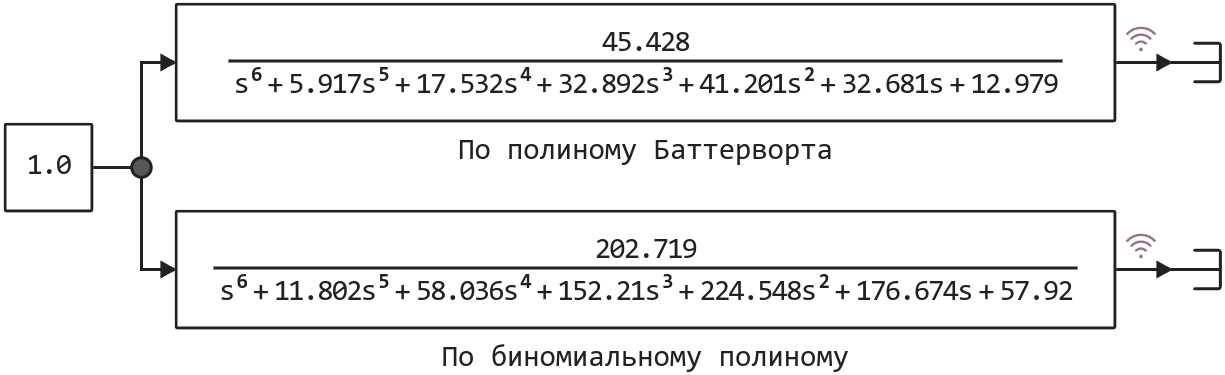
\includegraphics[height=0.13\textheight]{sources/task1_model.png}
    \caption*{Схема моделирования системы}
\end{figure}
К отчёту приложен файл \href{run:sources}{\texttt{task1.engee}}, содержащий эту схему. Симуляция проведена в среде моделирования и симуляции \href{https://start.engee.com/}{Engee}.\\[0.5em]
Теперь посмотрим на графики переходных характеристик для обоих типов распределения корней характеристического уравнения:
\begin{figure}[H]
    \centering
    \begin{minipage}{0.4\textwidth}
        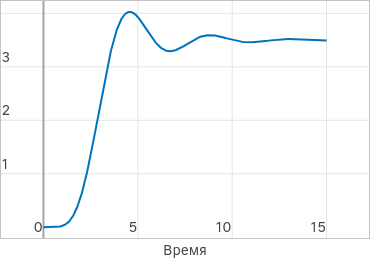
\includegraphics[width=\textwidth]{sources/task1_btw.png}
        \caption*{\centering График переходной характеристики\\для полинома Баттерворта}
    \end{minipage}
    \hspace{2em}
    \begin{minipage}{0.4\textwidth}
        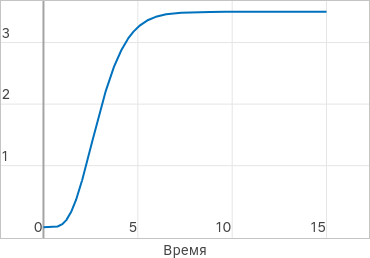
\includegraphics[width=\textwidth]{sources/task1_binom.png}
        \caption*{\centering График переходной характеристики\\для биномиального полинома}
    \end{minipage}
\end{figure}
Отмечу, что в обоих случаях переходные характеристики сходятся с течением времени к $k = 3.5$.

\addsection{Задание №2}
\addsubsection{Порядок выполнения работы}
Для каждого набора параметров $b_0, \ldots, b_m$ построить переходные характеристики системы с коэффициентами $a_0,\ldots,a_{n-1}$ и коэффициентом $b$, рассчитанными в предыдущем задании для биномиального распределения корней характеристического уравнения.\\[0.5em]
Первый набор параметров:
$$b_0 = b, \quad b_1 = 1.5.$$
Второй набор параметров:
$$b_0 = b, \quad b_1 = 0.1, \quad b_2 = 0.2, \quad b_3 = 0.4, \quad b_4 = 0.5, \quad b_5 = 0.2, \quad b_6 = 3.$$

% MARK: №2
\addsubsection{Выполнение работы}
Для первого набора параметров модель будет иметь следующий вид:
$$y^{(6)} + 11.802y^{(5)} + 58.036y^{(4)} + 152.21\dddot{y} + 224.548\ddot{y} + 176.674\dot{y} + 57.92 = 1.5\dot{g} + 202.719g.$$
Смоделируем систему и построим график переходной характеристики:
\begin{figure}[H]
    \centering
    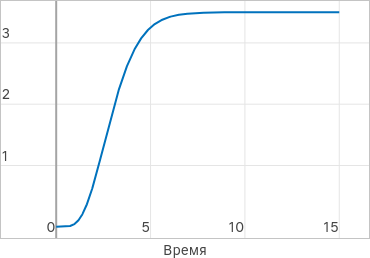
\includegraphics[width=0.4\textwidth]{sources/task2_1.png}
    \caption*{График переходной характеристики для первого набора параметров}
\end{figure}
Для второго набора параметров модель будет иметь следующий вид:
$$y^{(6)} + 11.802y^{(5)} + 58.036y^{(4)} + 152.21\dddot{y} + 224.548\ddot{y} + 176.674\dot{y} + 57.92 = 3g^{(6)} + 0.2g^{(5)} + 0.5g^{(4)} + 0.4\dddot{g} + 0.2\ddot{g} + 0.1\dot{g} + 202.719g.$$
Так же смоделируем систему и построим график переходной характеристики:
\begin{figure}[H]
    \centering
    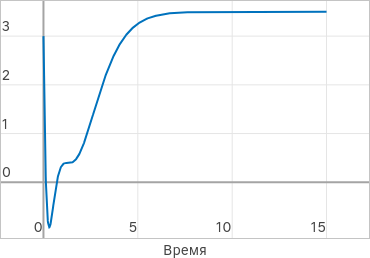
\includegraphics[width=0.4\textwidth]{sources/task2_2.png}
    \caption*{График переходной характеристики для второго набора параметров}
\end{figure}
Схема моделирования системы для обоих наборов параметров одинакова --- к отчёту приложен файл \href{run:sources}{\texttt{task2.engee}}, содержащий эту схему, симуляция которой проведена в среде моделирования и симуляции \href{https://start.engee.com/}{Engee}.

\addsection{Задание №3}
\addsubsection{Порядок выполнения работы}
Для набора параметров $b_0, \ldots, b_m$ и внешнего воздействия $g(t)$ построить реакцию системы с нулевыми начальными условиями и коэффициентами $a_0,\ldots,a_{n-1}$, рассчитанными в первом задании для биномиального распределения корней характеристического уравнения. Вывести графики $y(t)$ и $g(t)$.\\[0.5em]
Заданный набор параметров:
$$b_0 = 4.5, \quad b_1 = 0, \quad b_2 = 0.5, \quad g(t)=\cos{3t}$$

% MARK: №3
\addsubsection{Выполнение работы}
Имеем модель системы:
$$y^{(6)} + 11.802y^{(5)} + 58.036y^{(4)} + 152.21\dddot{y} + 224.548\ddot{y} + 176.674\dot{y} + 57.92 = 0.5\ddot{g} + 4.5.$$
Смоделируем систему и построим графики $y(t)$ и $g(t)$. Схема моделирования системы выглядит так:
\begin{figure}[H]
    \centering
    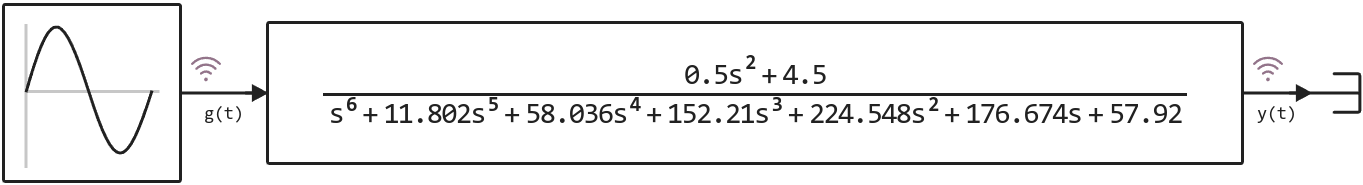
\includegraphics[width=0.5\textwidth]{sources/task3_model.png}
    \caption*{Схема моделирования системы}
\end{figure}
К отчёту приложен файл \href{run:sources}{\texttt{task3.engee}}, содержащий эту схему. Симуляция проведена в среде моделирования и симуляции \href{https://start.engee.com/}{Engee}.\newpage
Теперь посмотрим на графики $y(t)$ и $g(t)$:
\begin{figure}[H]
    \centering
    \begin{minipage}{0.4\textwidth}
        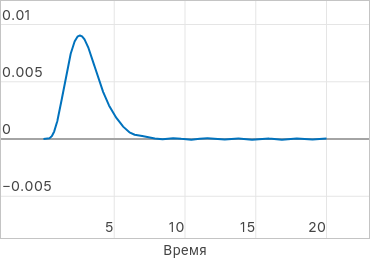
\includegraphics[width=\textwidth]{sources/task3_yt.png}
        \caption*{\centering График $y(t)$}
    \end{minipage}
    \hspace{2em}
    \begin{minipage}{0.4\textwidth}
        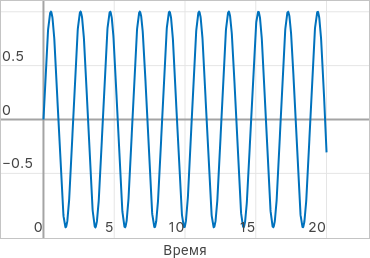
\includegraphics[width=\textwidth]{sources/task3_gt.png}
        \caption*{\centering График $g(t)$}
    \end{minipage}
\end{figure}

\addsection{Выводы}
В ходе выполнения лабораторной работы были изучены связь характера переходной характеристики, динамических свойств системы с размещением на комплексной плоскости нулей и полюсов передаточной функции. Были рассмотрены два типа распределения корней характеристического уравнения --- полином Баттерворта и биномиальный полином. Для каждого типа распределения были рассчитаны параметры системы и построены переходные характеристики. Также были рассмотрены два набора параметров и построены переходные характеристики для них. В конце была построена реакция системы на внешнее воздействие.

\end{document}